\chapter{Efecte terra. Ala.}
Un cop s'ha estudiat el comportament de l'ala sola, s'analitza el seu comportament sota les condicions d'efecte terra. L'efecte terra consisteix en el comportament que presenta l'ala quan es troba a una distància petita respecte el terra. En aquestes condicions, la presència d'una superfície sola força a la velocitat sobre el terra a mentenir-se paral·lela a aquest, quan en condicions normals no ho faria. Això provoca una variació del flux d'aire, que fa variar la sustentació i resistència aerodinàmica de l'ala.

En el cas plantejat, l'ala es troba a una distància de $h=\bar{c}$, i amb un angle d'atac respecte la velocitat de 6$^{\circ}$. A la figura \ref{GroundEffect} es pot veure un esquema d'aquest cas.

\begin{figure}[H]
	\centering
	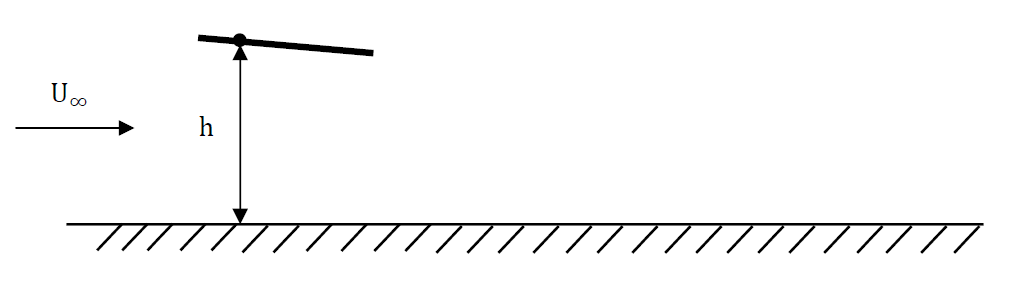
\includegraphics[scale=0.5]{./plots/GroundEffectWing.png}
	\caption{Esquema de la posició de l'ala sobre el terra}
	\label{GroundEffect}
\end{figure}

Concretament s'estudiarà la diferència del $C_{L}$ i del $C_{D}$, amb i sense presència d'efecte terra. Addicionalment, s'estudiarà com varien aquests valors en funció de l'allargament de l'ala.

\section{Algoritme}
\label{gndAlg}
Per tal de calcular l'efecte terra s'ha aplicat el mètode de les imatges. Amb aquesta finalitat s'ha afegit una ala simètrica respecte el terra obtenint així uns coeficients d'influència modificats respecte el cas sense efecte Terra. Aquesta modificació afegeix un cost computacional significatiu, ja que es tenen el doble d'elements que amb una ala sola. Pel que fa al càlcul de les circulacions i dels coeficients aerodinàmics, aquest no varia respecte de l'anterior apartat.


\section{Variació dels coeficients}

Agafant l'ala que ja s'ha descrit als apartats anteriors, sense torsió, i amb un angle d'atac de 6$^{\circ}$, es comparen els resultats dels coeficients aerodinàmics pel cas sense efecte terra, i pel cas amb efecte terra. Els resultats es poden veure a la taula \ref{NoGroundvsGround}.

\begin{table} [H]
	\centering
	\begin{tabular}{| c | c | c | c |}	
		\hline
		& $C_{L}$ & $C_{D}$ & $C_{m_{0}}$ \\
		\hline
		Sense efecte terra & 0.8273 & 0.0129 & -0.3737 \\
		\hline
		Amb efecte terra & 0.8895 & 0.0082 & -0.4051 \\
		\hline	
		Variació & 7.52\% & -36.43\% & 8.40\% \\
		\hline
	\end{tabular}
\caption{Variació dels coeficients amb i sense efecte terra} \label{NoGroundvsGround}
\end{table}
Com era d'esperar, la sustentació es veu lleugerament incrementada en presència de l'efecte Terra.
\section{Allargament}

Per veure la variació dels coeficients aerodinàmics amb l'allargament i l'efecte terra, s'ha pres el valor d'allargament de l'avió ($A_{0}$=26), i s'ha agafat l'espectre que va des de 0.75$A_{0}$ fins a 1.25$A_{0}$. Concretament s'han agafat 21 punts equidistribuïts, de manera que es té $A_{0}$ com a centre de l'espectre. Els resultats obtinguts han estat els següents.

\begin{figure}[H]
	\centering
	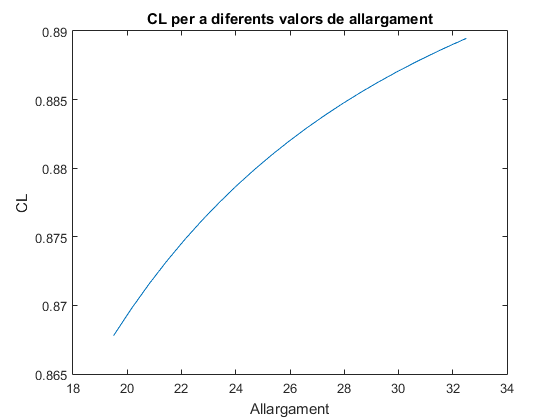
\includegraphics[]{./plots/CL_A}
	\caption{Variació del $C_{L}$ amb l'allargament amb efecte terra}
	\label{CL_A}
\end{figure}

\begin{figure}[H]
	\centering
	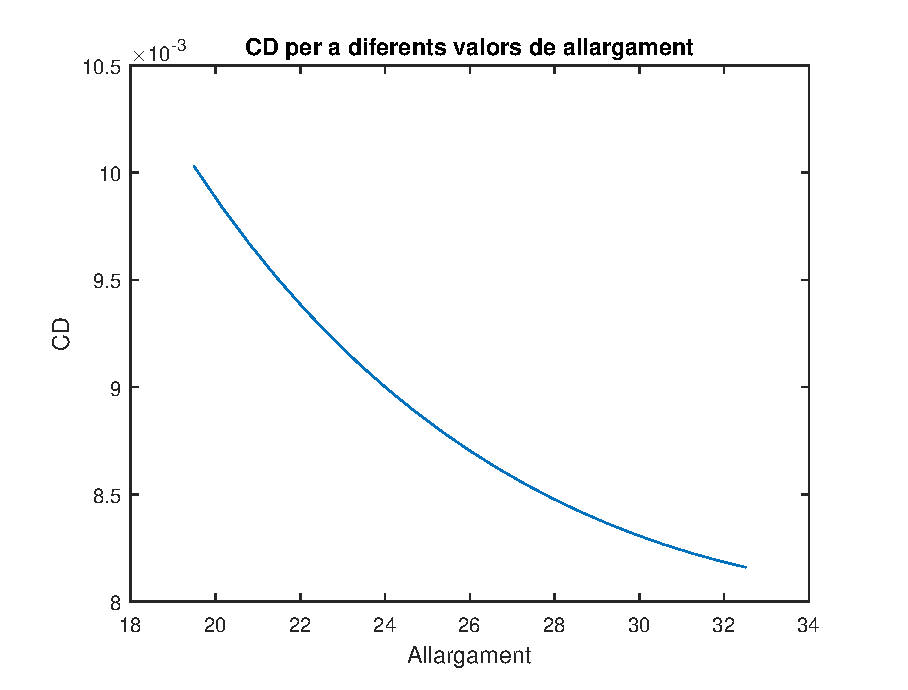
\includegraphics[]{./plots/CD_A}
	\caption{Variació del $C_{D}$ amb l'allargament amb efecte terra}
	\label{CD_A}
\end{figure}

\begin{figure}[H]
	\centering
	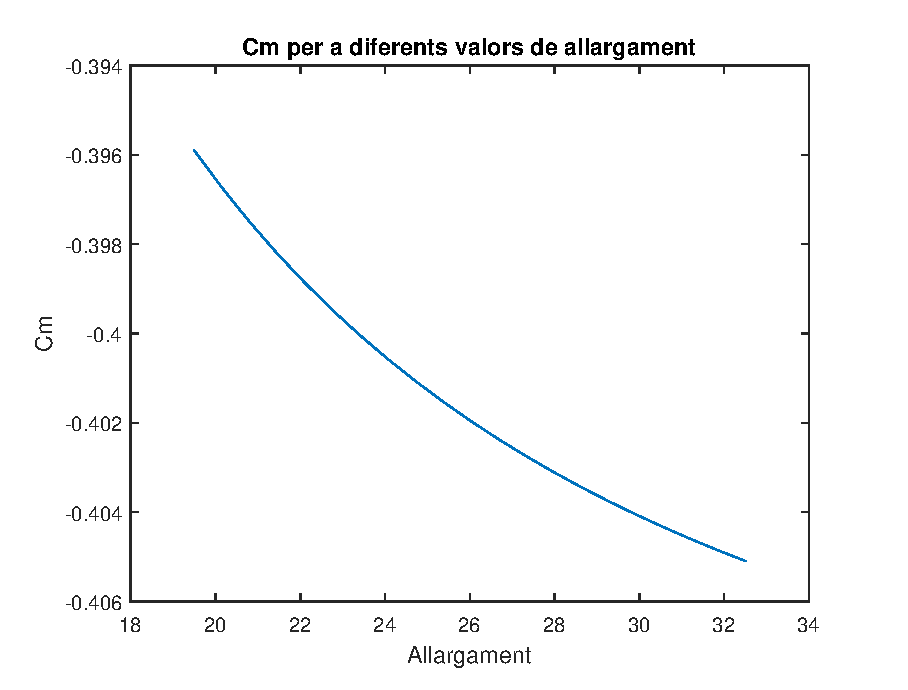
\includegraphics[]{./plots/Cm_A}
	\caption{Variació del $C_{m_{0}}$ amb l'allargament amb efecte terra}
	\label{Cm_A}
\end{figure}

Com es pot veure a les figures \ref{CL_A}, \ref{CD_A} i \ref{Cm_A}, el coeficient de sustentació augmenta amb l'allargament mentre que el coeficient de resistència aerodinàmica disminueix. Això és lògic, ja que en augmentar l'allargament, la punta de l'ala està més allunyada, de manera que hi ha una reducció en la velocitat induïda, cosa que provoca un augment del $C_{L}$. Pel mateix motiu, al ser menor la contribució dels vórtex de punta d'ala, hi ha una reducció de la resistència induïda. Finalment, degut a l'augment del coeficient de sustentació, augmenta també el coeficient de moment aerodinàmic respecte el caire d'atac.

Com es pot veure a les figures, aquesta variació dels coeficients no té un caràcter lineal, sinó que és assimptòtic. En el cas d'allargament infinit, una ala infinita, els coeficients aerodinàmics de l'ala esdevenen iguals als coeficients del perfil, que són els coeficients aerodiàmics sense efectes tridimensionals.